% !TEX root = ../thesis.tex
% [H] means put the figure HERE, directly when you input this code.
% Remove this to let LaTeX place the figure where it decides is best
\begin{figure}[H]
	\centering
	
% We use a figure width of 48.5% of the width of one line of text on 
% the page so there is some space between the images.
	\subfloat[Left image sub-caption.]{
		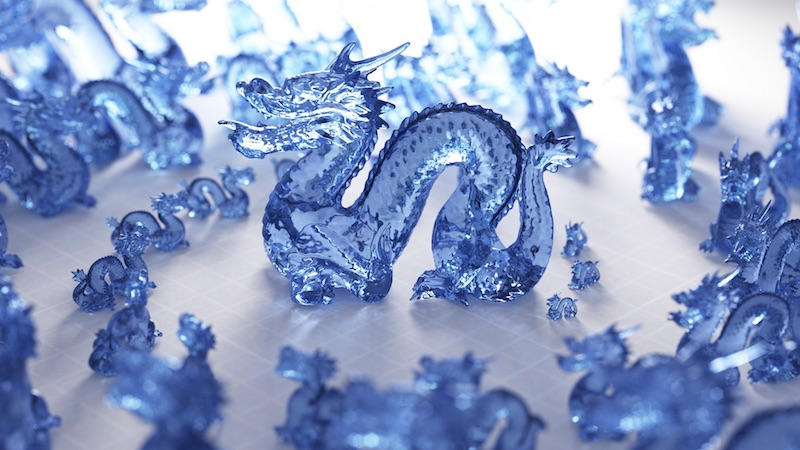
\includegraphics[width=0.485\textwidth]{dragon.jpg}\label{fig:example_2x1_a}
	}\hfill % Spacing between sub-figures displayed next to each other.
	\subfloat[Right image sub-caption.]{
		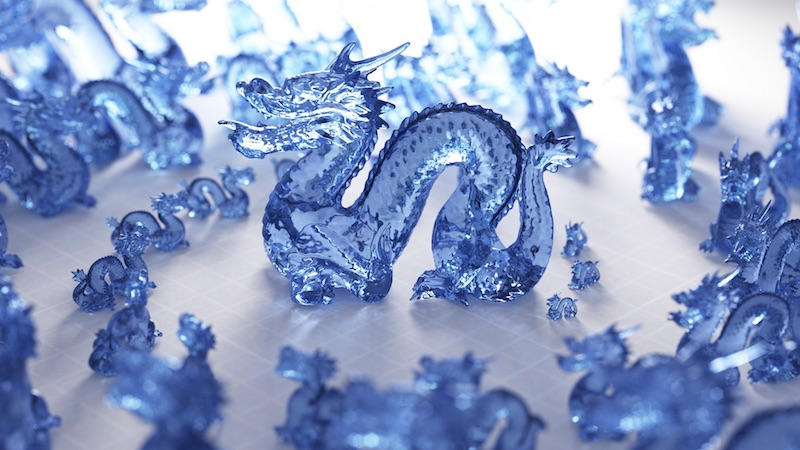
\includegraphics[width=0.485\textwidth]{dragon.jpg}\label{fig:example_2x1_b}
	}\\ % New line before caption.

% Caption is defined with a short and long version. The short version is shown in the 
% List of Figures section, and the long version is used directly with the figure. 	
	\caption[A demonstration of a 2x1 sub-figure layout.]{
Construct sub-figures from multiple image files in \LaTeX{} rather than in the image file itself.
This allows you to tweak the positioning and layout without having to modify the images.
It also allows for automatic formatting and numbering of captions and sub-captions.
Image of glass dragons rendered using Path Tracing \cite{whittle15_dragons}.
	
% Figure labels should be defined at the end of the caption to ensure proper numbering.
	\label{fig:example_2x1}
	}
	
\end{figure}